\section{Phase 1 - Planning and research phase}\label{sec:phase1}

After we had gotten in touch with Accenture and spoken with the supervisors and the product owner, the group had to make a few decisions regarding the project's direction.

An important choice for the project was to either build and train an AI model for the vehicles from scratch or use the existing model. Building a new AI model would provide a deeper understanding of the model we could utilize. Due to the time constraint, continuing with the existing model was more favorable. In addition, we believed that the project would have the potential to be too similar to the previous project.  Our group also had more prior experience with networking than with Raspberry Pi and AI. We, therefore, chose to use the AI model from the previous project. 

In this phase, we did not have access to the vehicle, nor the code, made by the prior bachelor group. However, there was a need for project planning and research before we could start developing our IoT system. The topics that needed to be researched were:

\begin{itemize}
\item What causes traffic jams and solutions to fix it.
\item IoT-systems and how they function with vehicles.
\item Planning and development methods that will fit our project
\end{itemize}

We also used the pre-project phase to get to know Accenture, their guidelines, and their workspace. Moreover, we participated in a "Design thinking"-workshop and made a work contract. 

%\subsection{Design thinking workshop}



\subsection{Choice of programming languages}
We chose to implement the client in Python and the server in C\#. The group before us had used Python for their Raspberry Pi vehicle, making Python a natural choice to extend the code from their project. Our group also had experience with networking in Python. Furthermore, the .NET ecosystem has well-developed solutions for creating IoT applications, microservices, and web applications \parencite{dotnet}. We had to write our server in C\#, to take advantage of these solutions. The server needed to be as efficient as possible, and C\# is also considered a fast programming language \parencite{csharp}. We also had some prior knowledge of coding in C\#.

\subsection{Internet of Things}

The Internet Of Things refers to physical objects that communicate using sensors, cameras, software, or other technologies connecting and exchanging data. This communication takes place over the internet or other communication forms. The number of connected IoT devices in the world is increasing, and it is becoming a big part of society \parencite{iot_analytics}. IoT has also been evolving in recent years due to other technologies becoming more accessible, such as machine learning and the 5G network.

IoT projects can, for instance, be applied in climate surveillance systems, energy, or transportation. In this thesis we will explore the possibilities of using IoT in transportation, more specifically in personal automobiles. The convergence of these fields is more commonly known as IoV, Internet of Vehicles. An IoV system is a distributed system for wireless communication and information exchange between vehicles through agreed-upon communication protocols \parencite{chinese_iov}. The system could potentially integrate functionality for dynamic information exchange, vehicle control and smart traffic management. In our thesis, we will explore these possibilities on a small scale.

\subsection{Preventing traffic congestions for a one-lane road}\label{sec:traffic_congestion}

Traffic congestion, also known as traffic jams, is when a long line of vehicles moves slowly or has stopped moving altogether. Traffic jams can create frustration and disrupt nearby local environments with sound and gas emissions \parencite{traffic_congestion_pollution}. Many factors can cause traffic congestion, such as:

poorly designed roads, not wide enough roads, traffic light patterns, and accidents \parencite{traffic_congestion}.

With this in mind, we started by focusing on a simple scenario: when a car drastically reduces its speed or completely stops on a single-lane road.

This scenario will lead to the vehicles behind needing to slow down drastically as well. This phenomenon is called traffic jam shockwave \parencite{traffic_shockwave}. To prevent this, we propose a solution where cars reduce their velocity before they reach the destination of where the shockwave started. For this to happen, a server could keep track of the cars' positions and send information to the vehicles behind, when required. 

We came up with an idea on how the server and cars should interact. First, the car would connect to the server and provide information about its current speed, weight, width, and length. The server would use this information to keep track of all the cars' positions on the road. The cars would send information to the server if their velocity changed. This message would trigger an event on the server where it would command all the cars behind to slow down accordingly. \figref{fig:diagramfirst} shows a flow chart of a potential simulation of this solution:

\begin{figure}[h!]
	\centering
	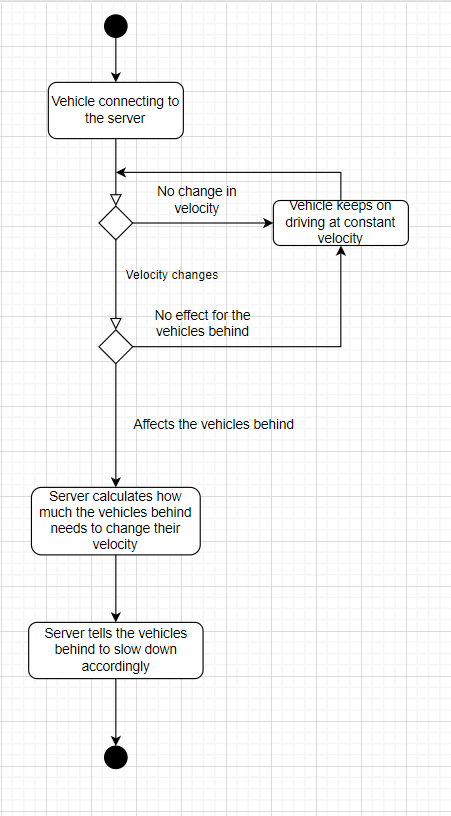
\includegraphics[width=0.9\linewidth]{figures/flow_diagram_first}
	\caption[Flow diagram server]{This figure shows the flow diagram of our first proposed solution. }
	\label{fig:diagramfirst}
\end{figure}
\clearpage